%# -*- coding:utf-8 -*-
\documentclass[10pt,aspectratio=169,mathserif]{beamer}		
%设置为 Beamer 文档类型,设置字体为 10pt,长宽比为16:9,数学字体为 serif 风格

%%%%-----导入宏包-----%%%%
\usepackage{zju}			%导入 zju 模板宏包
\usepackage{ctex}			%导入 ctex 宏包,添加中文支持
\usepackage{amsmath,amsfonts,amssymb,bm}   %导入数学公式所需宏包
\usepackage{color}			 %字体颜色支持
\usepackage{graphicx,hyperref,url}
\usepackage{metalogo}	% 非必须
\usepackage{ragged2e}
\usepackage{wrapfig}
\usepackage{caption}
%% 上文引用的包可按实际情况自行增删
%%%%%%%%%%%%%%%%%%
\usepackage{fontspec}
\usepackage{xeCJK}
% \setCJKmainfont{Source Han Sans SC}
\setbeamertemplate{caption}[numbered] % 图片添加编号


\beamertemplateballitem		%设置 Beamer 主题

%%%%------------------------%%%%%
\catcode`\。=\active         %或者=13
\newcommand{。}{.}				
%将正文中的“。”号转换为“.”。中文标点国家规范建议科技文献中的句号用圆点替代
%%%%%%%%%%%%%%%%%%%%%

%%%%----首页信息设置----%%%%
\title[间断有限元方法的算法设计与应用]{间断有限元方法的算法设计与应用}	
%%%%----标题设置


\author[鲁硕]{
  鲁硕 \\ \medskip
  {\small \url{lushuo@zju.edu.cn}} \\
}
%%%%----个人信息设置
  
\institute[IOPP]{
  信息与计算科学 \\ 
  浙江大学}
%%%%----机构信息

\date[\today]{
  \today}
%%%%----日期信息
  
\begin{document}

\begin{frame}
	\titlepage
\end{frame}				%生成标题页


\begin{frame}
	%%  	\frametitle{提纲}
	\tableofcontents
\end{frame}				%生成提纲页

\section{研究背景与意义}
\begin{frame}
	\frametitle{研究背景与意义}
	\begin{itemize}
		\item 半导体是一种电导率在绝缘体至导体之间的物质或材料。半导体器件利用此特性在电子技术、清洁能源、制造业和自动化等许多领域具有重要意义。半导体宏观数学模型则是现代半导体工业的重要研究课题之一,它不仅为为半导体材料、微电子配件等相关领域
		      的许多技术问题提供了理论上必要的解释,提供对器件行为和性能的预测和分析,利于半
		      导体材料开发和优化。
		\item LDG算法具有良好的h-p自适应性,出色的并行效率,因为它们在本质上是非常局部的。此外,这些方法具有优秀的可证明非线性稳定性。
	\end{itemize}

\end{frame}
\section{预备知识}
\begin{frame}
	\frametitle{介绍}
	\begin{itemize}
		\item 基础符号
		      $I_j = (x_{j-\frac{1}{2}},x_{j+\frac{1}{2}}),j=1,2,\cdots,N$是计算域I的一个划分。$\Delta x_j = x_{j+\frac{1}{2}}-x_{j-\frac{1}{2}},x_j = \frac{1}{2}(x_{j-\frac{1}{2}}+x_{j+\frac{1}{2}}), h = \max\{\sup\limits_{j} \Delta x_j\}$。有限维计算空间$V_h = V_h^k = \{z:z|_{I_j} \in P^k(I_j)\}$。

		      定义$(u_h)^+_{j+\frac{1}{2}} = u_h(x^+_{j+\frac{1}{2}})$和$(u_h)^-_{j+\frac{1}{2}} = u_h(x^-_{j+\frac{1}{2}})$。用$[u_h]_{j+\frac{1}{2}} = (u_h)^+_{j+\frac{1}{2}} - (u_h)^-_{j+\frac{1}{2}}$和$(\bar{u}_h)_{j+\frac{1}{2}}=\frac{1}{2}((u_h)^+_{j+\frac{1}{2}}+(u_h)^-_{j+\frac{1}{2}})$来表示$u_h$在每个单元边界点的跳跃和平均值。
	\end{itemize}
\end{frame}
\section{离散方法}
\subsection{空间离散方法}
\begin{frame}[allowframebreaks]
	\frametitle{空间离散方法}
	DG 法就是想找到$V_h$一组基的系数,进而得到解。考虑简单的问题
	\begin{equation*}
		\begin{cases}
			u_x = f,0\leq x \leq 1 \\
			u(0) = a,
		\end{cases}
	\end{equation*}
	$\int_{I_j}vu_x = \int_{I_j}vf$
	由分步积分得
	\begin{equation*}
		-\int_{I_j}uv_x\mathrm{d}x+u_{j+\frac{1}{2}}v_{j+\frac{1}{2}}-u_{j-\frac{1}{2}}v_{j-\frac{1}{2}} = \int_{I_j}vf\mathrm{d}x
	\end{equation*}
	假设u是准确解,$u_h$是数值解。对于任意可微的v上述等式都成立。对上式求解得到的解就是数值解,也就是上式可以写作
	\begin{equation*}
		-\int_{I_j}u_h v_x\mathrm{d}x+u_{j+\frac{1}{2}}v_{j+\frac{1}{2}}-u_{j-\frac{1}{2}}v_{j-\frac{1}{2}} = \int_{I_j}vf\mathrm{d}x
	\end{equation*}
	为了将DG法适用于含有高阶空间导数的方程,如
	\begin{equation}
		u_t = u_{xx}
	\end{equation}
	令$v = u_x$得到
	\begin{align}
		u_t - v_x = 0, \\
		v - u_x = 0.
	\end{align}
	LDG法的想法是找到$u_h,v_h\in V_h$使得$\forall w,z\in V_h$,我们有
	\begin{align}
		\int_{I_j}u_t w\rm{d}x + \int_{I_j}v_h w_x dx - \hat{v}_{j+1/2} w^-{j+1/2} + \hat{v}_{j-1/2}w^+{j-1/2} = 0, \label{scheme:LDG} \\
		\int_{I_j}v_h z d x + \int_{I_j}u_h z_x dx  - \hat{u}_{j+1/2}z^-_{j+1/2} + \hat{u}_{j-1/2}z^+_{j-1/2} = 0. \label{scheme:LDG aux}
	\end{align}
	其中$\hat{u}_{j+1/2} = 1/2(u^-_{j+1/2} + u^+_{j+1/2}),\hat{v}_{j+1/2} = 1/2(v^-_{j+1/2} + v^+_{j+1/2})$。

\end{frame}
\subsection{时间离散方法}
\begin{frame}[allowframebreaks]
	\frametitle{总变差不增龙格库塔法(TVD RK)}
	离散情况下的总变差是
	$$
		TV(u^n) = TV(u(\cdot ,t^n)) = \sum_j |u^n_{j+1} - u^n_j|
	$$
	其中$u^n_j = u(x_j,t^n)$.

	TV不增,即
	$$
		TV(u^{n+1}) \leq TV(u^n).
	$$
	RK通常有形式
	\begin{align}
		u^{(i)} = \sum^{i-1}_{k=0}(a_{ik}u^{(k)} + \Delta t \beta_{ik}L(u^{(k)})),\quad i = 1,\ldots,m,\label{eq:RK} \\
		u^{(0)} = u^n, \quad u^{(m)} = u^{n+1}. \nonumber
	\end{align}
	\begin{block}{引理}
		当$a_{ik} \geq 0, \beta_{ik} \geq 0$,RK法\eqref{eq:RK}在CFL条件下是TVD,其中$CFL = \min \limits_{i,k}\frac{\beta_{ik}}{\alpha_{ik}} \Delta t $,即
		\begin{equation}
			\Delta t \leq CFL\Delta t_1
		\end{equation}
	\end{block}

	\begin{block}{最优三阶TVD RK法}
		\begin{align*}
			u^{(1)} & = u^n + \Delta t L(u^n),                                                \\
			u^{(2)} & = \frac{1}{2}u^n + \frac{1}{4}u^{(1)} + \frac{1}{4}\Delta L(u^{(1)})),  \\
			u^{n+1} & = \frac{1}{3}u^n + \frac{2}{3}u^{(2)} + \frac{2}{3}\Delta t L(u^{(2)}).
		\end{align*}
		其中$\alpha_{ik} \geq 0, \beta_{ik}\geq 0$,CFL=1.
	\end{block}
\end{frame}

\begin{frame}[allowframebreaks]
	\frametitle{IMEX RK法}
	该方法的想法是隐性处理线性扩散部分,显性处理非线性耦合漂移项来节省计算成本,同
	时依然追求无条件稳定性,即时间步长可以取小于给定常数的任意值。
\end{frame}
\section{物理模型}
\subsection{DD模型}
\begin{frame}[allowframebreaks]
	\frametitle{DD模型}
	DD(drift-diffusion)模型
	\begin{block}{DD模型}
		\begin{align}
			n_t - (\mu En)_x = \tau \theta n_{xx}, \label{equation:DD} \\
			\phi_{xx} = \frac{e}{\epsilon}(n - n_d),  \label{equation:poisson}
		\end{align}
		其中$x \in (0,1)$,第一个方程具有周期边界条件,势方程$\phi(0,t) = 0, \phi(1,t) = v_{bias}$具有Dirichlet边界条件。泊松方程\eqref{equation:poisson}是电势方程,$E = -\phi_x$代表电场。

		在系统\eqref{equation:DD}-\eqref{equation:poisson},未知变量是电子浓度n和电势$\phi$。$m_0$是电子有效质量,k是Boltzmann常数,e是电子电荷,$\mu$是迁移率,$T_0$是晶格温度,$\tau = \frac{m_0 \mu}{e}$是松弛参数,$\theta = \frac{k}{m_0}T_0$,$\epsilon$是节电常数,$n_d$是掺杂,这是一个给定的函数。
	\end{block}
	令$q = \sqrt{\tau \theta }n_x$,因此等式\eqref{equation:DD}可以写作
	\begin{align}
		n_t - (\mu E n)_x - \sqrt{\tau \theta}q_x = 0, \\
		q - \sqrt{\tau \theta}n_x = 0,                 \\
		E_x = -\frac{e}{\epsilon}(n - n_d),            \\
		E = - \phi_x.
	\end{align}
	用测试函数$v,w,r,z \in V_h^k$分别乘以上述方程,再对所有包含空间导数的部分进行公式化的分部积分来得到
	\begin{align}
		\int_{I_j} n_t v \rm{d}x + \int_{I_j}(\mu En + \sqrt{\tau \theta}q)v_x\rm{d} x          \nonumber                                                                                                             \\
		- (\mu En + \sqrt{\tau \theta}q)_{j+\frac{1}{2}}v_{j+\frac{1}{2}}^- +(\mu En + \sqrt{\tau \theta}q)_{j-\frac{1}{2}}v_{j-\frac{1}{2}}^+ = 0, \label{weakForm:1}                                                \\
		\int_{I_j} qw\rm{d}x + \int_{I_j}\sqrt{\tau \theta} n w_x \rm{d}x - \sqrt{\tau \theta} n_{j+\frac{1}{2}}w_{j+\frac{1}{2}}^- + \sqrt{\tau \theta} n_{j-\frac{1}{2}}w_{j-\frac{1}{2}}^+ = 0, \label{weakForm:2} \\
		-\int_{I_j}Er_x\rm{d}x + E_{j+\frac{1}{2}}r_{j+\frac{1}{2}}^- - E_{j-\frac{1}{2}}r_{j-\frac{1}{2}}^+ = -\frac{e}{\epsilon}\int_{I_j}(n-n_d)r\rm{d}x,                                       \label{weakForm:3} \\
		\int_{I_j} Ez \rm{d}x - \int_{I_j}\phi z_x \rm{d}x + \phi_{j+\frac{1}{2}}z_{j+\frac{1}{2}}^- - \phi_{j-\frac{1}{2}}z_{j-\frac{1}{2}}^+ = 0,\label{weakForm:4}
	\end{align}
	其中$ j=1,\cdots,N$,$v,w,r,z \in V_h$。
	\begin{block}{DD 另一种 LDG 格式}
		\begin{align}
			 & \int_{I_{j}}\left(n^{h}\right)_{t} v d x+\int_{I_{j}}\left(\mu E^{h} n^{h}+\sqrt{\tau \theta} q^{h}\right) v_{x} d x            \nonumber                                                                                                                 \\
			 & \quad-\left(\mu \widehat{E^{h} n^{h}}+\sqrt{\tau \theta} \hat{q}^{h}\right)_{j+\frac{1}{2}} v_{j+\frac{1}{2}}^{-}+\left(\mu \widehat{E^{h} n^{h}}+\sqrt{\tau \theta} \hat{q}^{h}\right)_{j-\frac{1}{2}} v_{j-\frac{1}{2}}^{+}=0, \label{eq:DDaReformLDGa} \\
			 & \int_{I_{j}} q^{h} w d x+\int_{I_{j}} \sqrt{\tau \theta} n^{h} w_{x} d x-\sqrt{\tau \theta} \hat{n}_{j+\frac{1}{2}}^{h} w_{j+\frac{1}{2}}^{-}+\sqrt{\tau \theta} \hat{n}_{j-\frac{1}{2}}^{h} w_{j-\frac{1}{2}}^{+}=0,            \label{eq:DDaReformLDGb} \\
			 & E_{x}^{h}=\tilde{E}_{x}^{h}=-\frac{e}{\varepsilon}\left(n^{h}-n_{d}\right),   \label{eq:DDaReformLDGc}                                                                                                                                                    \\
			 & E^{h}=\tilde{E}^{h}-v_{\text {bias }}=\int_{0}^{x}-\frac{e}{\varepsilon}\left(n^{h}-n_{d}\right) d x+E_{0}-v_{\text {bias }},\label{eq:DDaReformLDGd}
		\end{align}
		其中,$E_{0}=E^{h}(0)=\int_{0}^{1}\left(\int_{0}^{x} \frac{e}{\varepsilon}\left(n^{h}-n_{d}\right) d s\right) d x$。这里的“hat”表示数值通量。
	\end{block}
\end{frame}
\subsection{HF模型}
\begin{frame}[allowframebreaks]
	\frametitle{HF模型}
	\begin{block}{HF模型}
		\begin{align}
			n_{t}+J_{x}=0, \quad x \in(0,1), \label{eq:HF} \\
			\phi_{xx} = \frac{e}{\epsilon}(n - n_d). \label{eq:DDP}
		\end{align}
		Poisson电场方程\eqref{eq:DDP}带有周期边界条件,其中$J=J_{h y p}+J_{v i s}$,
		而
		$$
			\begin{gathered}
				J_{h y p}=-\mu n E+\tau \mu\left(\frac{e}{\varepsilon}\right) n(-\mu n E+\omega) \\
				J_{v i s}=-\tau\left(n\left(\theta+2 \mu^{2} E^2\right)\right)_{x}+\tau \mu E(\mu n E)_{x} .
			\end{gathered}
		$$
		这里,$\omega=\left.(\mu n E)\right|_{x=0}$取常数。未知量与DD模型中相同:电子浓度$n$和电势$\phi$。
	\end{block}
	定义$C_{1}=\frac{\tau \mu e}{\varepsilon}$,$C_{2}=\frac{\tau \mu^{2} e}{\varepsilon}=\mu C_{1}$和$C_{3}=\frac{\tau \mu e \omega}{\varepsilon}=\omega C_{1}$,$q=\sqrt{\tau \theta+\tau \mu^{2} E^{2}} n_{x}=\left(\sqrt{\tau \theta+\tau \mu^{2} E^{2}} n\right){x}-\left(\sqrt{\tau \theta+\tau \mu^{2} E^{2}}\right){x} n$,我们可以将方程$~\eqref{eq:HF}$改写为以下系统
	\begin{align}
		 & n_{t}+\left(-\left(3 C_{2} E n_{d}+\mu E-C_{3}\right) n+2 C_{2} E n^{2}-\sqrt{\tau \theta+\tau \mu^{2} E^{2}} q\right)_{x}=0, \label{eq:HFRewrittenca} \\
		 & q=\left(\sqrt{\tau \theta+\tau \mu^{2} E^{2}} n\right)_{x}-\left(\sqrt{\tau \theta+\tau \mu^{2} E^{2}}\right)_{x} n.\label{eq:HFRewrittencb}
	\end{align}
	我们分别用测试函数$v, w \in V_{h}^{k}$乘以方程~\eqref{eq:HFRewrittenca}-\eqref{eq:HFRewrittencb},并对涉及空间导数的所有项进行形式上的分部积分,得到以下弱形式
	\begin{align}
		 & \int_{I_{j}} n_{t} v d x+\int_{I_{j}}\left(3 C_{2} E n_{d}+\mu E-C_{3}\right) n v_{x} d x -\left(3 C_{2} E n_{d} n+\mu E n-C_{3} n\right)_{j+\frac{1}{2}} v_{j+\frac{1}{2}}^{-}                                                                                       \nonumber           \\
		 & +\left(3 C_{2} E n_{d} n+\mu E n-C_{3} n\right)_{j-\frac{1}{2}} v_{j-\frac{1}{2}}^{+}  -\int_{I_{j}} 2 C_{2} E n^{2} v_{x} d x+2 C_{2}\left(E n^{2}\right)_{j+\frac{1}{2}} v_{j+\frac{1}{2}}^{-}-2 C_{2}\left(E n^{2}\right)_{j-\frac{1}{2}} v_{j-\frac{1}{2}}^{+}           \nonumber    \\
		 & +\int_{I_{j}} \sqrt{\tau \theta+\tau \mu^{2} E^{2}} q v_{x} d x -\left(\sqrt{\tau \theta+\tau \mu^{2} E^{2}} q\right)_{j+\frac{1}{2}} v_{j+\frac{1}{2}}^{-}+\left(\sqrt{\tau \theta+\tau \mu^{2} E^{2}} q\right)_{j-\frac{1}{2}} v_{j-\frac{1}{2}}^{+}=0  \label{eq:HFRewrittenWeakForma} \\
		 & \int_{I_{j}} q w d x+\int_{I_{j}} \sqrt{\tau \theta+\tau \mu^{2} E^{2}} n w_{x} d x+\int_{I_{j}}\left(\sqrt{\tau \theta+\tau \mu^{2} E^{2}}\right)_{x} n w d x    \nonumber                                                                                                               \\
		 & -\left(\sqrt{\tau \theta+\tau \mu^{2} E^{2}} n\right)_{j+\frac{1}{2}} w_{j+\frac{1}{2}}^{-}+\left(\sqrt{\tau \theta+\tau \mu^{2} E^{2}} n\right)_{j-\frac{1}{2}} w_{j-\frac{1}{2}}^{+}=0 .\label{eq:HFRewrittenWeakFormb}
	\end{align}
	将上述方程中的精确解$n, q$替换为它们在$V_{h}^{k}$中的数值近似$n^{h}, q^{h}$,注意到数值解$n^{h}$和$q^{h}$在单元边界上不连续,然后将单元边界上的项替换为合适的数值通量,我们得到LDG格式:
	\begin{align}
		 & \int_{I_{j}} n_{t}^{h} v d x+\int_{I_{j}}\left(3 C_{2} E^{h} n_{d}+\mu E^{h}-C_{3}\right) n^{h} v_{x} d x                                                                   \nonumber                                                                                                                                                                                               \\
		 & -\left(3 C_{2} E^{h} n_{d}+\mu E^{h}-C_{3}\right)_{j+\frac{1}{2}} \hat{n}_{j+\frac{1}{2}}^{h} v_{j+\frac{1}{2}}^{-} +\left(3 C_{2} E^{h} n_{d}+\mu E^{h}-C_{3}\right)_{j-\frac{1}{2}} \hat{n}_{j-\frac{1}{2}}^{h} v_{j-\frac{1}{2}}^{+}                                                                                                                                   \nonumber \\
		 & -\int_{I_{j}} 2 C_{2} E^{h}\left(n^{h}\right)^{2} v_{x} d x+2 C_{2}\left(E^{h} \widehat{\left(n^{h}\right)^{2}}\right)_{j+\frac{1}{2}} v_{j+\frac{1}{2}}^{-}-2 C_{2}\left(E^{h} \widehat{\left(n^{h}\right)^{2}}\right)_{j-\frac{1}{2}} v_{j-\frac{1}{2}}^{+} \nonumber                                                                                                             \\
		 & +\int_{I_{j}} \sqrt{\tau \theta+\tau \mu^{2}\left(E^{h}\right)^{2}} q^{h} v_{x} d x \nonumber                                                                                                                                                                                                                                                                                       \\
		 & -\left(\sqrt{\tau \theta+\tau \mu^{2}\left(E^{h}\right)^{2}} \hat{q}^{h}\right)_{j+\frac{1}{2}} v_{j+\frac{1}{2}}^{-}+\left(\sqrt{\tau \theta+\tau \mu^{2}\left(E^{h}\right)^{2}} \hat{q}^{h}\right)_{j-\frac{1}{2}} v_{j-\frac{1}{2}}^{+}=0,             \label{eq:HFRewrittenLDGa}                                                                                                \\
		 & \int_{I_{j}} q^{h} w d x+\int_{I_{j}} \sqrt{\tau \theta+\tau \mu^{2}\left(E^{h}\right)^{2}} n^{h} w_{x} d x+\int_{I_{j}}\left(\sqrt{\tau \theta+\tau \mu^{2}\left(E^{h}\right)^{2}}\right)_{x} n^{h} w d x                        \nonumber                                                                                                                                         \\
	\end{align}
	\begin{equation}
		-\left(\sqrt{\tau \theta+\tau \mu^{2}\left(E^{h}\right)^{2}} \hat{n}^{h}\right)_{j+\frac{1}{2}} w_{j+\frac{1}{2}}^{-}+\left(\sqrt{\tau \theta+\tau \mu^{2}\left(E^{h}\right)^{2}} \hat{n}^{h}\right)_{j-\frac{1}{2}} w_{j-\frac{1}{2}}^{+}=0 .\label{eq:HFRewrittenLDGb}
	\end{equation}
	数值电场$E^{h}$的求解与之前一样。
\end{frame}

\section{误差分析}
\begin{frame}[allowframebreaks]
	\frametitle{误差分析}
	由于篇幅限制,具体证明过程此处不列出。
	\begin{itemize}
		\item 	DD模型LDG格式
		      \begin{theorem}
			      设$n, q$是问题\eqref{equation:DD}-\eqref{equation:poisson}的精确解,具有足够光滑且有界导数。设$n^{h}, q^{h}$是半离散LDG格式\eqref{eq:DDaReformLDGa}-\eqref{eq:DDaReformLDGb}的数值解,并将相应的数值误差记为$e_{u}=u-u_{h}(u=n, q)$。如果有限元空间$V_{h}^{k}$是$k \geq 1$次分段多项式,则对于足够小的$h$,有以下误差估计成立:
			      $$
				      \left\|n-n^{h}\right\|_{L^{\infty}\left(0, T ; L^{2}\right)}+\left\|q-q^{h}\right\|_{L^{2}\left(0, T ; L^{2}\right)} \leq C h^{k+\frac{1}{2}}
			      $$
			      其中常数$C$依赖于最终时间$T$、$k$、$\|n\|_{L^{\infty}\left(0, T ; H^{k+1}\right)}$、$\left\|n_{x}\right\|_{0, \infty}$、$\left\|n_{d}\right\|_{0, \infty}$。
		      \end{theorem}
		\item HF模型LDG格式
		      \begin{theorem}
			      设$n, q$是问题~\eqref{eq:HFRewrittenca}-\eqref{eq:HFRewrittencb}的精确解,具有足够光滑且有界导数。设$n^{h}, q^{h}$是半离散LDG格式~\eqref{eq:HFRewrittenLDGa}-\eqref{eq:HFRewrittenLDGa}的数值解,并将相应的数值误差记为$e_{u}=u-u_{h}(u=n, q)$。如果有限元空间$V_{h}^{k}$是$k \geq 2$次分段多项式,则对于足够小的$h$,有以下误差估计成立:

			      $$
				      \left\|n-n^{h}\right\|_{L^{\infty}\left(0, T ; L^{2}\right)}+\left\|q-q^{h}\right\|_{L^{2}\left(0, T ; L^{2}\right)} \leq C h^{k+\frac{1}{2}}
			      $$

			      其中常数$C$依赖于最终时间$T$、$k$、$\|n\|_{L^{\infty}\left(0, T ; H^{k+1}\right)}$、$\left\|n_{x}\right\|_{0, \infty}$、$\left\|n_{d}\right\|_{0, \infty}$以及导数$\left|a^{\prime}\right|$和$\left|b^{\prime}\right|$的界。
		      \end{theorem}
		\item DD模型 三阶IMEX LDG格式
		      \begin{theorem}
			      令$n^m,q^m$是问题~\eqref{weakForm:1}-\eqref{weakForm:4}在时间层级m的精确解,它们足够光滑且有有界导数。令$n_h^m,q_h^m$是三阶IMEX LDG格式。如果有限元空间$V_h^k$是k$(k\geq  0)$阶间断多项式,那么对于足够小的h,存在正常数C与h无关,使得下列误差估计成立
			      \begin{equation}
				      ||n-n_h||_{L^{\infty}(0,T;L^2)} + ||q - q_h||_{L^2(0,T;L^2)} \leq C(h^{k+1} + (\Delta t)^3)
			      \end{equation}
			      其中C依赖于最终时间T,k,反常数$C_2$, $||n||_{L^{\infty}(0,T;H^{k+1})}$,$||n_x||_{L^{\infty}}$和$||E||_{L^{\infty}}$。
		      \end{theorem}
		\item DD模型 Dirichlet边界条件
		      \begin{theorem}\label{theo:6.1}
			      令$n,q$是问题~\eqref{weakForm:1}-\eqref{weakForm:4}的精确解,它们足够光滑且导数有界。令$n_h,q_h$是半离散LDG格式的数值解。定义对应的数值误差$e_h = u-u_h(u = n,q)$。如果有限元空间$V_h^k$是k$(k\geq  0)$阶间断多项式,那么对于足够小的h,下列误差估计成立
			      \begin{equation}
				      ||n-n_h||_{L^{\infty}(0,T;L^2)} + ||q - q_h||_{L^2(0,T;L^2)} \leq Ch^{k+\frac{1}{2}}
			      \end{equation}
			      其中C依赖于最终时间T,k,反常数$C_2$, $||n||_{L^{\infty}(0,T;H^{k+1})}$,$||n_x||_{L^{\infty}}$和$||E||_{L^{\infty}}$。
		      \end{theorem}
		      如果我们选择边界处的数值通量
		      \begin{equation}
			      (\hat{q}_h)_{\frac{1}{2}} = (q_h^+)_{\frac{1}{2}} + c_0[n_h]_{\frac{1}{2}}. \label{numbericalFlux:optimal}
		      \end{equation}
		      我们可以得到下列最优误差估计。
		      \begin{equation}
			      ||n-n_h||_{L^{\infty}(0,T;L^2)} + ||q - q_h||_{L^2(0,T;L^2)} \leq C h^{k+1}
		      \end{equation}
		      其中C依赖于最终时间T,k,反常数$C_2$, $||n||_{L^{\infty}(0,T;H^{k+1})}$,$||n_x||_{L^{\infty}}$和$||E||_{L^{\infty}}$。
	\end{itemize}
\end{frame}
\section{数值模拟}
\begin{frame}[allowframebreaks]
	\frametitle{数值模拟}
	具体参数受限于篇幅省略。

	\begin{minipage}{.4\textwidth}
		\centering
		图\ref{fig:DD&HF simu}描绘出DD和HF模型的模拟结果,上面两张图片比较了DD模型的模拟结果,$\mu=\mu\left(n_{d}\right)$ with $\mu=0.75$。下面两张图比较DD模型和HF模型的结果, $\mu=\mu\left(n_{d}\right)$。
	\end{minipage}
	\hspace{0.05\textwidth}
	\begin{minipage}{.5\textwidth}
		\centering
		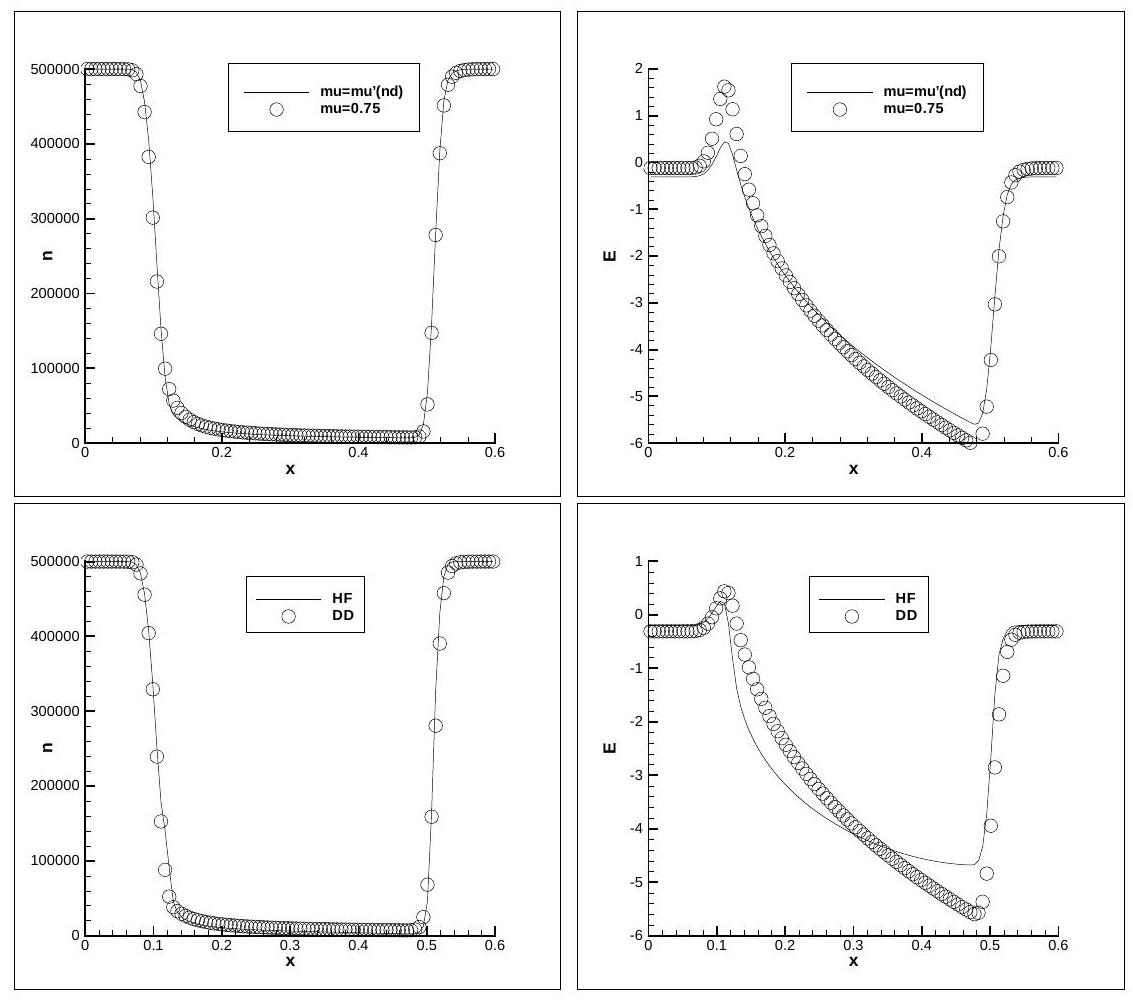
\includegraphics[width=\textwidth]{figure/DD&HF simu}
		\captionof{figure}{[0,0.6] with 100 mesh cells. Left: density $n\left(10^{12} \mathrm{~cm}^{-3}\right)$; right: electric field $E(\mathrm{~V} / \mathrm{um})$}
		\label{fig:DD&HF simu}
	\end{minipage}
	三阶IMEX LDG方案的模拟结果与TVD RK时间离散化的结果以供比较。基选择缩放的Legendre多项式基。

	数值模拟显示,无论选择 $h$ 的值如何(在 $[0,0.6]$ 中的100或200网格单元格),方案都是稳定的。 代码在网格细化期间产生数值收敛结果(为节省空间,未显示网格细化结果),正如本文所示的理论结果所预期的。

	从表\ref{tab:1}和表\ref{tab:2}中,我们可以看到,使用第三阶 IMEX LDG 方案,我们可以使用更大的时间步长,从而显著节省CPU时间。 IMEX 方案因此是研究像 DD 这样的模型描述正确物理规律的适用性的一个可靠而有效的工具。

	\begin{table}
		\caption{在 $[0,0.6]$ 中具有100个网格单元的第三阶 RK LDG 和第三阶 IMEX LDG 方法达到稳态所需的时间步长 $\Delta t$,时间步数 $n t$,时间 $t$,和 CPU 时间}
		\label{tab:1}
		\centering

		\begin{tabular}{|c|c|c|c|c|c|c|}
			\hline
			           & Third order EX-RK    & \multicolumn{5}{|c|}{Third order IMEX}                                                                                     \\
			\hline
			$\Delta t$ & $1.688 \mathrm{E}-5$ & $1.2 \mathrm{E}-3$                     & $1.8 \mathrm{E}-3$ & $2.4 \mathrm{E}-3$ & $3.0 \mathrm{E}-3$ & $3.6 \mathrm{E}-3$ \\
			\hline
			$n t$      & 44063                & 711                                    & 476                & 356                & 286                & 239                \\
			\hline
			$t$        & 0.7436               & 0.8532                                 & 0.8568             & 0.8544             & 0.8580             & 0.8604             \\
			\hline
			CPU time   & 58.8904              & 4.6332                                 & 3.4008             & 2.5272             & 2.0592             & 1.482              \\
			\hline
		\end{tabular}

	\end{table}
	\begin{table}
		\caption{在$[0,0.6]$中具有200个网格单元的三阶RK LDG法和三阶 IMEX LDG方法达到稳态所需的时间步长$\Delta t$,时间步数 $n t$,时间 $t$,和 CPU 时间。}
		\label{tab:2}
		\centering
		\begin{tabular}{|c|c|c|c|c|c|c|}
			\hline
			           & Third order EX-RK   & \multicolumn{5}{|c|}{Third order IMEX}                                                                                     \\
			\hline
			$\Delta t$ & $4.22 \mathrm{E}-6$ & $1.2 \mathrm{E}-3$                     & $1.8 \mathrm{E}-3$ & $2.4 \mathrm{E}-3$ & $3.0 \mathrm{E}-3$ & $3.6 \mathrm{E}-3$ \\
			\hline
			$n t$      & 176081              & 727                                    & 480                & 360                & 298                & 249                \\
			\hline
			$t$        & 0.7431              & 0.8724                                 & 0.864              & 0.864              & 0.894              & 0.8964             \\
			\hline
			CPU time   & 202.3957            & 7.5349                                 & 5.5224             & 4.3680             & 3.4476             & 3.276              \\
			\hline
		\end{tabular}
	\end{table}
	\begin{figure}
		\centering
		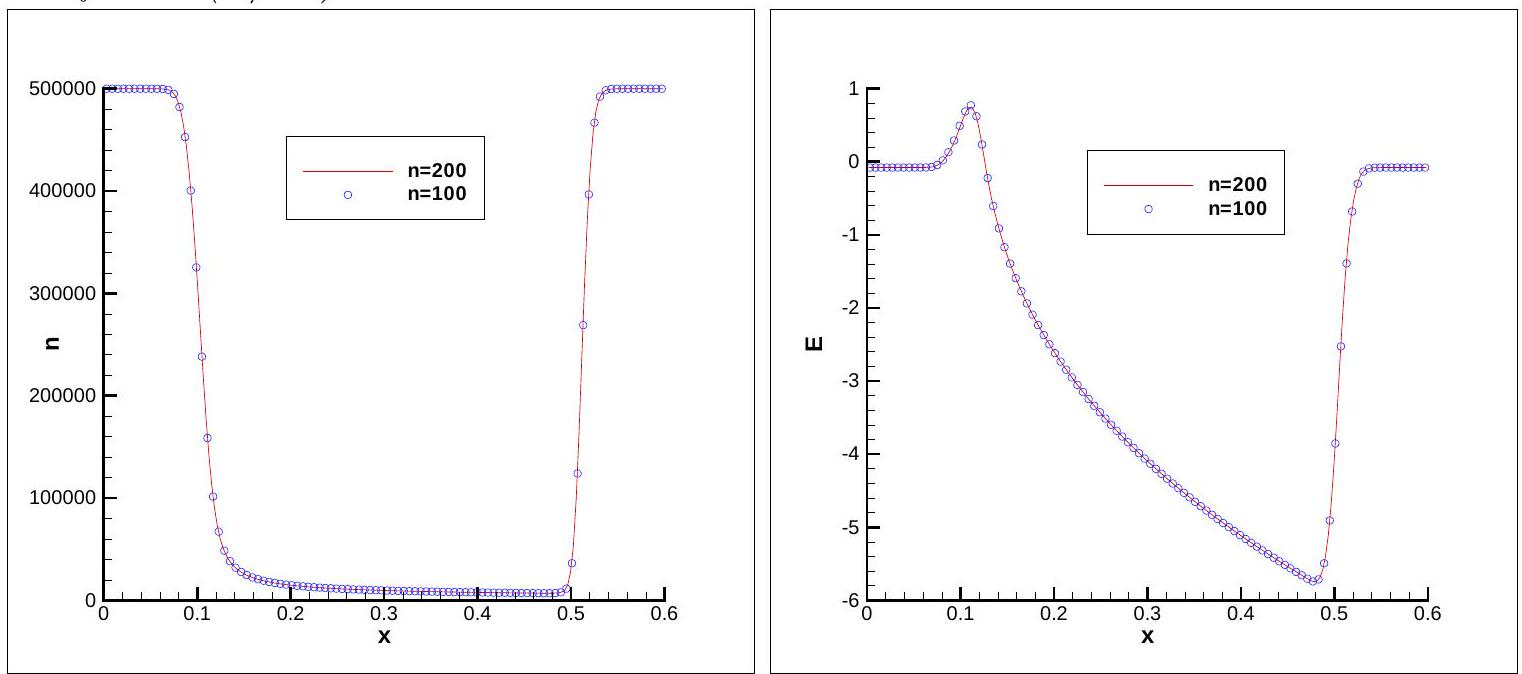
\includegraphics[width=0.8\textwidth]{figure/numbericalsimulationresulttranslation}
		\caption{在 $[0,0.6]$ 有100或200个网格单元, $\Delta t=1.2 E-3$。 左边:密度 $n\left(10^{12} \mathrm{~cm}^{-3}\right)$;右边:电场 $E$ (V/um)。}
		\label{fig:numbericalsimulationresulttranslation}
	\end{figure}
\end{frame}
\begin{frame}
	\frametitle{鸣谢}
	\Huge
	\begin{center}
		谢谢!
	\end{center}
\end{frame}
\end{document}